\documentclass[mathserif,t]{beamer}
%http://tex.stackexchange.com/questions/105613/footer-in-beamer. Check this out. Frankfurt template.
%http://tex.stackexchange.com/questions/39345/piecewise-highlighting-in-beamer-presentation
%https://joerglenhard.wordpress.com/2011/08/01/beamer-customization-colors/
\usepackage{amssymb,bm,mathtools,amsmath}                                                      
\usepackage{graphicx,caption,float}
\usepackage[UKenglish]{isodate} % for: \today                             
\cleanlookdateon                % for: \today                             

\def\wl{\par\vspace{\baselineskip}\noindent}                             
\def\beginmyfig{\begin{figure}[ht]\begin{center}}                          
\def\endmyfig{\end{center}\end{figure}}                                   

\def\prodl#1#2#3{\prod\limits_{#1=#2}^{#3}}                               
\def\suml#1#2#3{\sum\limits_{#1=#2}^{#3}}                                 
\def\ds{\displaystyle}                                                    
\def\tbf#1{\textbf{#1}}
\def\inv{^{\raisebox{.2ex}{$\scriptscriptstyle-1$}}}
\def\pm{^{\raisebox{.2ex}{$\scriptscriptstyle\prime$}}}
\def\norm#1{\left\lVert#1\right\rVert}

% My Beamer Stuff
  \geometry{vmargin=0.3in} % Formating the top bar
  \newcommand{\m}[1]{\mathbf{\bm{#1}}} % Serif bold math

  % My Color Stuff
  \usepackage{xcolor} % http://en.wikibooks.org/wiki/LaTeX/Colors
                      % http://latexcolor.com/
    \definecolor{grey}{rgb}{0.15, 0.15, 0.15} % Sets default color. CHANGE THIS!
    \definecolor{pumpkin}{rgb}{1.0, 0.46, 0.09}
    \definecolor{darktan}{rgb}{1.0, 0.66, 0.07}
    \definecolor{coral}{rgb}{1.0, 0.5, 0.31}
    \definecolor{burlywood}{rgb}{0.98, 0.82 0.6}
    \pagecolor{grey}% Sets the bar color.

  \def\mylitecolor{pumpkin}         % Bullet Color.       CHANGE THIS!
  \def\mycolor{\color{pumpkin}}     % Frame Title Color.  CHANGE THIS!
  \def\mydarkcolor{\color{pumpkin}} % Figure Color.       CHANGE THIS!
    \def\frametitle#1{\vspace{-.32in{\mycolor\textbf{\Large#1}}}}
    \setbeamercolor{itemize item}{fg=\mylitecolor}
    \setbeamercolor{enumerate item}{fg=\mylitecolor}
    \setbeamercolor{itemize subitem}{fg=\mylitecolor}
    \setbeamercolor{itemize subsubitem}{fg=\mylitecolor}
    \setbeamercolor{title}{fg=\mylitecolor}
    \setbeamercolor{footlinecolor}{bg=black!93,fg=\mylitecolor}
    \setbeamercolor{author}{fg=burlywood}
    \setbeamercolor{date}{fg=burlywood}
    \setbeamercolor{institute}{fg=burlywood}

    \usepackage[T1]{fontenc}
    \DeclareCaptionFont{figcol}{\mydarkcolor} %color of the word Figure: in figure captions
    \captionsetup{
      font=scriptsize,
      labelfont={bf,figcol,scriptsize}%,textfont={black}
    }
  \def\hline{ \textcolor{grey}{\hrulefill}\\ }

  % Beamer Footer Stuff:
  %http://tex.stackexchange.com/questions/26476/add-footer-text-to-all-slides-in-beamer
  %http://tex.stackexchange.com/questions/105613/footer-in-beamer
  \beamertemplatenavigationsymbolsempty
  \setbeamertemplate{footline}{
    \hbox{
      \hspace{-.17cm}
      \begin{beamercolorbox}[ht=2mm,dp=8.2mm,leftskip=.3cm,rightskip=.3cm]{footlinecolor}%
        \insertauthor\hfill\insertshorttitle\hfill\insertframenumber/\inserttotalframenumber
      \end{beamercolorbox}
    }
  }

%%%%% Example for embedding images: %%%%%%%%%%%%%%%%%%%%%%%%%%%%%%%%%%%%%%%%%%%%%%%%%%%%%%%%%%%%
%%%\frame{
%%%  \frametitle{How to embed images:}
%%%  \beginmyfig
%%%    \includegraphics[scale=.21]{path/to/file.pdf}
%%%    \caption{Put Caption Here}
%%%  \endmyfig
%%%  \footnote{\tiny \url{https://www.luiarthur.github.com} }
%%%}
% End of Header. Start below beamer below. %%%%%%%%%%%%%%%%%%%%%%%%%%%%%%%%%%%%%%%%%%%%%%%%%%%%%

% defs for this assignment:

\begin{document}
% My Title: {
  \def\mytitle{\textbf{ Bayesian Nonparametric Spatial Modeling with Dirichlet Process Mixing }}
  \title[Spatial DP]{\mytitle}
  \author[Arthur Lui]{Arthur Lui}
  \institute{
    AMS\\
    UC Santa Cruz
  }
  {
    \setbeamercolor{background canvas}{bg=grey}
    \frame{\titlepage}
  }
%}

\frame{ \frametitle{Data} \beginmyfig \includegraphics[scale=.5]{../graphs/july1985.pdf} \endmyfig }
\frame{ \frametitle{Data} \beginmyfig 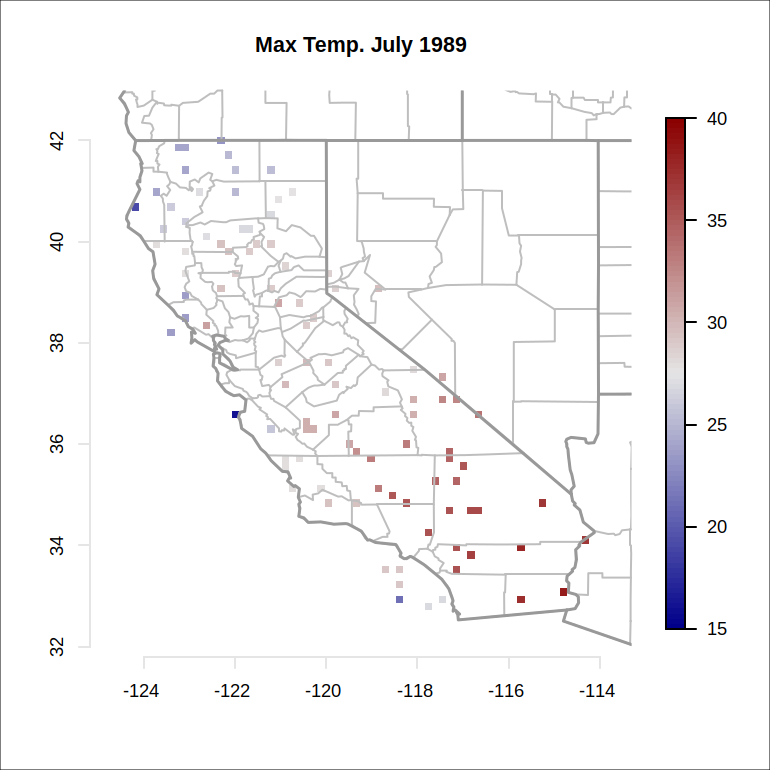
\includegraphics[scale=.5]{../graphs/july1989.pdf} \endmyfig }
\frame{ \frametitle{Data} \beginmyfig \includegraphics[scale=.5]{../graphs/july1994.pdf} \endmyfig }
\frame{ \frametitle{Data} \beginmyfig \includegraphics[scale=.5]{../graphs/july1999.pdf} \endmyfig }
\frame{ \frametitle{Data} \beginmyfig \includegraphics[scale=.5]{../graphs/july2004.pdf} \endmyfig }

\frame{ %
  \frametitle{Spatial DP}
  \vspace{5mm}
  \begin{itemize}
    \item The spatial DP is defined as a random process over $D$ \[
        G_D = \sum_{l=1}^\infty \omega_l \delta_{\theta_l,D}
      \] which is centered at $G_{0D}$.
  \vspace{10mm}
    \item This process is denoted $G_D \sim \text{SDP}(\alpha,G_{0D})$.
  \vspace{10mm}
    \item Random process $G_D$ can be centered at a stationary Gaussian process, 
      and be nonstationary. 
  \end{itemize}
}


\frame{ %2
  \frametitle{Model}
  \vspace{0mm}
  \[
    \begin{array}{rclcl}
      %\m y_t &|& \m\theta_t,\beta,\tau^2 &\overset{ind.}{\sim}&\text{Normal}_n(\m\theta_t+ \m x_t\beta,
      \m y_t &|& \m\theta_t,\beta,\tau^2 &\overset{ind.}{\sim}&\text{N}_n(\m\theta_t+ \m{1_n}\beta,
      ~\tau^2\m I_n), ~~_{t=1,...,T}\\
      \m\theta_t &|& G^{(n)} &\overset{i.i.d.}{\sim}& G^{(n)}, ~~_{t=1,...,T} \\
      G^{(n)} &|& \alpha, \sigma^2, \phi &\sim& \text{DP}(~\alpha,~\text{N}_n(\m 0_n,\sigma^2H_n(\phi)) ~) \\
      \\
              && \beta, \tau^2 &\sim& \text{N}(m,s^2) \times \text{IGamma}(a_{\tau^2}=2,b_{\tau^2}) \\
              && \alpha &\sim& \text{Gamma}(a_\alpha,b_\alpha) \\
              && \sigma^2 &\sim& \text{IGamma}(b_{\sigma^2}=2,b_{\sigma^2}) \\
              && \phi &\sim& \text{Uniform}(0,b_\phi) \\
    \end{array}
  \]
  where 
  \begin{itemize}
    \item $H_n(\phi)$ is a covariance function, for example, the exponential
      covariance function with decay parameter $\phi$. (i.e.  $(H_n(\phi))_{ij}
      = \exp\left\{-\phi~\norm{s_i-s_j}\right\}$.) \\
    \item $\m y_t(s)$ is the average daily maximum temperature ($^oC$) at location $s$ for replicate $t$.
    %\item $\m y_t$ are the station-measured Ozone levels for the $t^{th}$ replicate.
    %\item $\m x_t$ are a average CMAQ value of the 3 locations nearest to the prediction location for the
    %  $t^{th}$ replicate.
  \end{itemize}
}

\frame{ %3
  \frametitle{Posteriors}
  \[\def\arraystretch{1.4}
    \begin{array}{rclcl}
      \beta &|& \m y, \m\theta, \tau^2  &\sim& \text{N}(
        \frac{\tau^2m + s^2\sum_{t=1}^T\sum_{i=1}^n(y_{it}-\theta_{it})}{\tau^2+Tns^2},
        \frac{s^2\tau^2}{\tau^2+Tns^2}) \\
      \tau^2 &|& \m y, \m\theta, \beta  &\sim& \text{IG}(a_{\tau^2}+\frac{nT}{2},
      b_{\tau^2}+\frac{\sum_{t=1}^T (\m\mu_t-\beta \m1_n)'(\m\mu_t-\beta \m1_n)}{2})\\
      %p(\sigma^2 &|& \m\theta_t^*, T^*, \m y, \sigma^2) &\propto& [\sigma^2]\prod_{t=1}^{T^*}
      %  ~\text{N}_n(\m\theta_t^* | \m 0_n,\sigma^2H_n(\phi)) ~)\\
      \sigma^2 &|& \m\theta^*, T^*, \m y, \sigma^2 &\sim& \text{IG}(a_{\sigma^2}+\frac{nT^*}{2},
        %b+\frac{\sum_{t=1}^{T^*}\m\theta^*'Hn^{-1}(\phi)\m\theta^*}{2})\\
      b_{\sigma^2}+\frac{\sum_{t=1}^{T^*}\m\theta_t^{*'} H_n^{-1}(\phi)\m\theta_t^*}{2})\\
      %p(\phi &|& \m\theta_t^*, T^*, \m y, \sigma^2) &\propto& \prod_{t=1}^{T^*} 
      %  ~\text{N}_n(\m\theta_t^* |\m 0_n,\sigma^2H_n(\phi)) ~)\\
      p(\phi &|& \m\theta^*, T^*, \m y, \sigma^2) &\propto& 
      [\phi]|H_n(\phi)|^{-T^*/2} \exp\left(-\frac{\sum_{t=1}^{T^*}\m\theta_t^{*'} H_n^{-1}(\phi)\m\theta_t^*}{2\sigma^2}\right)\\
      \eta &|& \alpha, \m y &\sim& \text{Beta}(\alpha+1,T)\\
      p(\alpha &|& T^*, \m y) &=& (\epsilon)~\gamma(\alpha | a_\alpha+T^*, b_\alpha-\log(\eta)) +\\
               &&&&(1-\epsilon)~\gamma(\alpha | a_\alpha+T^*-1, b_\alpha-\log(\eta))\\
    \end{array}
  \]
  where $\m\mu_t=\m{y_t -\theta_t} $, $\eta$ is an auxiliary variable introduced
  to make the prior for $\alpha$ conjugate, $\gamma$ is the gamma density
  function with the mean and rate parameterization, and 
  $\epsilon = \ds\frac{a_\alpha +T^* - 1}{ n(b_\alpha-\log(\eta)) + a_\alpha +T^* -1}$.
}

\frame{ %4
  \frametitle{Posterior for $\m\theta$}
  \def\mm{\m{y_t}-\m{1_n}\beta}
  \[\def\arraystretch{1.4}
    \begin{array}{rllcl}
      \m\theta_t &|& y_t,\beta,\tau^2,\sigma^2,\phi &\sim& \text{N}_n(\tau^{-2}\m\Lambda(\mm), \m\Lambda)\\
                 && q0 &=& |\Lambda|^{1/2} \\
                 %&&&& \times \exp\left\{.5\tau^{-2}(\mm)'(\m{I_n}-\tau^{-2}\m\Lambda)(\mm)\right\}\\
                 &&&& \times \exp\left\{\frac{(\mm)'(\m{I_n}-\tau^{-2}\m\Lambda)(\mm)}{2\tau^2}\right\}\\
                 &&&& \times [(2\pi\tau^2\sigma^2)^{n/2} |\m H_n(\phi)|^{1/2}]^{-1}\\
    \end{array}
  \]
  where $\m\Lambda = [\tau^{-2}\m I_n + \sigma^{-2} \m H_n^{-1}(\phi)]^{-1}$.
}


\frame{
  \frametitle{Posterior Predictive}
  \beginmyfig
    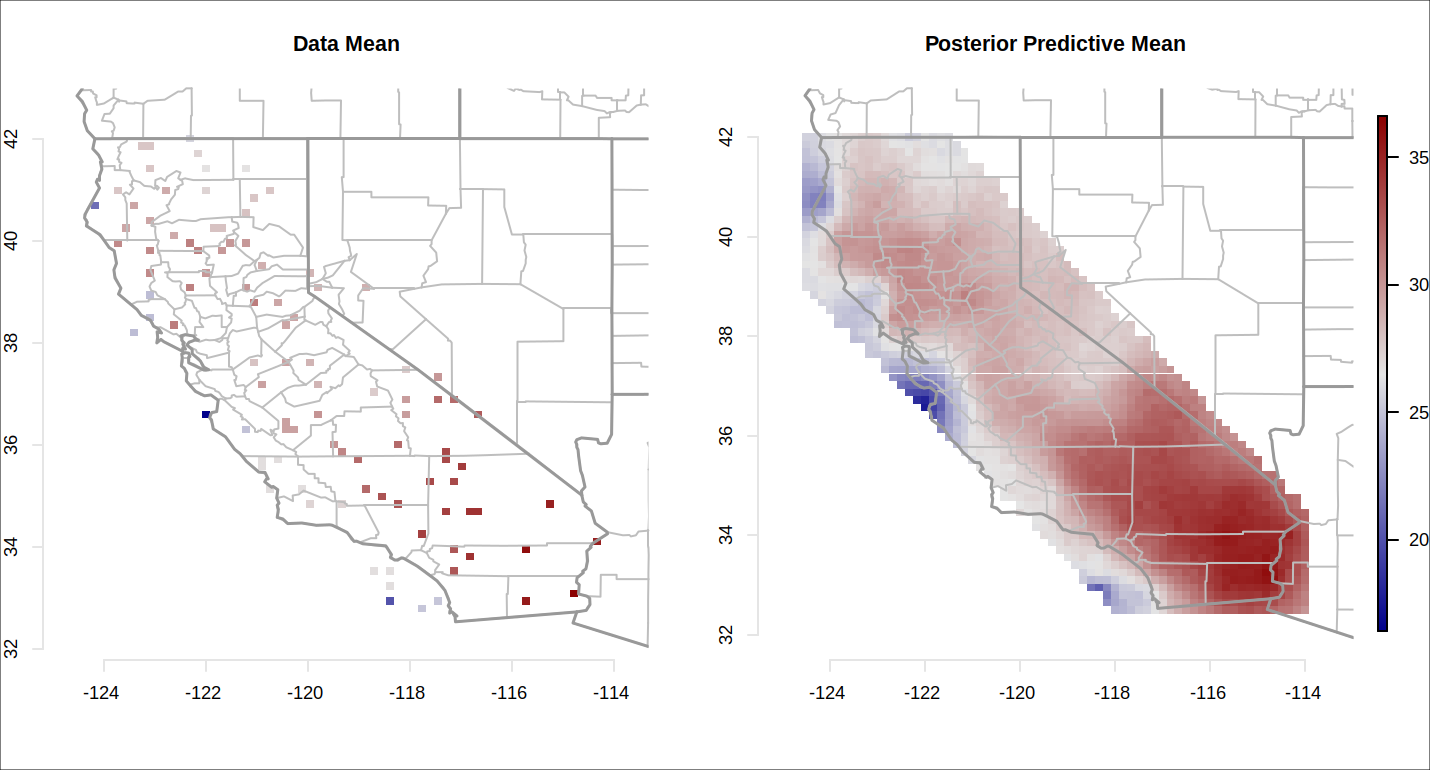
\includegraphics[scale=.35]{../graphs/postpredmean.pdf}
  \endmyfig
}
\frame{
  \frametitle{Posterior Predictive}
  \beginmyfig
    \includegraphics[scale=.35]{../graphs/postpredvar.pdf}
  \endmyfig
}


% End Frame:
{\setbeamercolor{background canvas}{bg=grey}
  \frame{
    \frametitle{}
    \vspace{25mm}
    \begin{center}
      \color{pumpkin}\Huge \textbf{Questions}
    \end{center} 
  }
}

\end{document}
% To compile:
%  $ pdflatex *.tex; pdflatex *.tex
